\documentclass[12pt,twoside,book]{article}
\usepackage{docmute}

\input{../settings}

\begin{document}

%%%%%%%%%%%%%%%%%%%%%%%%%%%%%%%%%%%%%%%%%%%%%%%%%%%%%%%%%%%%%%%%%%%%%%%%%%%%%%%
\section{Models with WIMPs}
\setcounter{equation}{0}
%%%%%%%%%%%%%%%%%%%%%%%%%%%%%%%%%%%%%%%%%%%%%%%%%%%%%%%%%%%%%%%%%%%%%%%%%%%%%%%

\vskip 0.1in

There are several examples of the models that contain WIMP DM
candidates.  In this section, two of them \rem{Really?} are briefly
reviewed.  \rem{EWIMP and WIMP??}

%%%%%%%%%%%%%%%%%%%%%%%%%%%%%%%%%%%%%%%%%%%%%%%%%%%%%%%%%%%%%%%%%%%%%%%%%%%%%%%
\subsection{Minimally supersymmetric standard model}
%%%%%%%%%%%%%%%%%%%%%%%%%%%%%%%%%%%%%%%%%%%%%%%%%%%%%%%%%%%%%%%%%%%%%%%%%%%%%%%

\rem{Summary of SUSY particle names somewhere}

\begin{figure}[b]
  \centering
  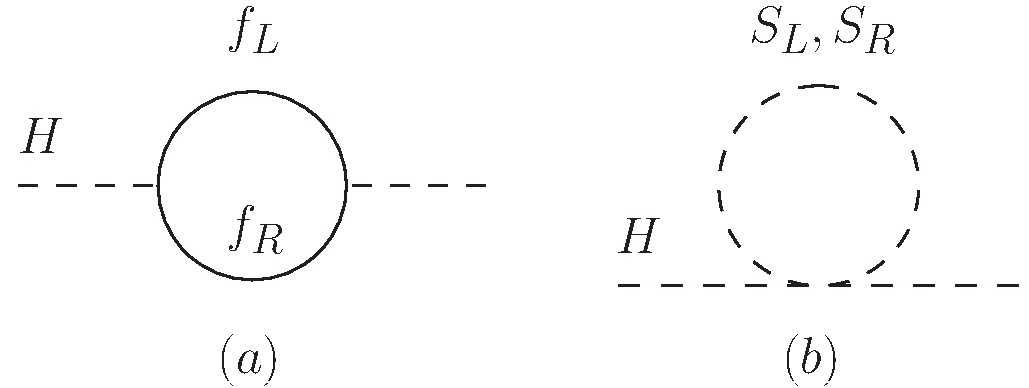
\includegraphics[width=0.6\hsize]{loop_correction.pdf}
  \caption{One-loop correction to the Higgs mass from (a) a Weyl fermion $f$ and (b) a complex scalar $S$.}
  \label{fig:loop_correction}
\end{figure}

The minimally supersymmetric standard model (MSSM) is the simple extension of the SM with $\mathcal{N} = 1$ supersymmetry (SUSY).
\footnote{
  For a brief review of the $\mathcal{N} = 1$ SUSY, see Sec.~\ref{sec:susy}.
}
One of the motivations to introduce SUSY is to solve the so-called hierarchy (or naturalness) problem \cite{Weinberg:1975gm,Gildener:1976ai,Susskind:1978ms} in the SM.
The problem is related to the quantum correction to the SM Higgs boson mass from heavy new physics particles.
For example, we can consider the one-loop correction to the Higgs mass from a Weyl fermion $f$ and a complex scalar $S$ as illustrated in Fig.~\ref{fig:loop_correction}.
The corrections to the Higgs mass is given by
\begin{align}
  \Delta m_h^2 &= -\frac{|\lambda_f|^2}{8 \pi^2} \left[
  \Lambda_{\mathrm{UV}}^2 - 2 m_f^2 \ln \left( \frac{\Lambda_{\mathrm{UV}}}{m_f} \right)
  + \cdots \right] & &\mathrm{(fermion)}, \label{eq:delmh_f}\\
  \Delta m_h^2 &= \frac{\lambda_S}{16 \pi^2} \left[
  \Lambda_{\mathrm{UV}}^2 - 2 m_S^2 \ln \left( \frac{\Lambda_{\mathrm{UV}}}{m_S} \right)
  + \cdots \right] & &\mathrm{(scalar)}, \label{eq:delmh_S}
\end{align}
\rem{Check this!}
where $\lambda_f$ and $m_f$ are the Higgs-fermion coupling constant and the fermion mass, respectively, and $\lambda_S$ and $m_S$ are those for the scalar $S$.
We take the cut-off scale of the theory to be $\Lambda_{\mathrm{UV}}$ to regularize the otherwise divergent loop integral and neglect the lower order terms of $\Lambda_{\mathrm{UV}}$.
Eqs.~\eqref{eq:delmh_f} and \eqref{eq:delmh_S} show the quadratic dependence of $\Delta m_H^2$ on $\Lambda_{\mathrm{UV}}$, which means that the Higgs mass is sensitive to the energy scale of the beyond the SM physics.
However, there is at least one extremelly high energy scale physics in the nature, gravity at the Planck scale $M_{\mathrm{pl}} \sim 10^{18 \hyphen 19}\,\mathrm{GeV}$.
By substituting $\Lambda_{\mathrm{UV}} = M_{\mathrm{pl}}$ in Eqs.~\eqref{eq:delmh_f} and \eqref{eq:delmh_S} and assuming $\lambda_f \sim \lambda_S \sim \mathcal{O} (1)$, we notice that orders-of-magnitude fine-tuning is required to obtain the correct Higgs mass $m_h = 125.10\,\mathrm{GeV}$ \cite{Tanabashi:2018oca}, which is unnatural.

SUSY provides a nice solution to this fine-tuning problem.
As is summarized in Appendix~\ref{sec:susy}, \rem{summarize later} each Weyl fermion in a supersymmetric model has two complex scalars with the same mass $m_f = m_S$.
In addition, their coupling constants should have a relationship $|\lambda_f|^2 = \lambda_S$ due to the fact that $\lambda_S$ is a coupling constant in the F-term potential sourced by a superpotential term proportional to $\lambda_f$. \rem{description of F-term and D-term}
By using both equations and summing the corrections \eqref{eq:delmh_f} and \eqref{eq:delmh_S} with factor of two multiplied to the latter, we obtain a result independent of the cut-off scale $\Lambda_{\mathrm{UV}}$ without fine-tuning.
This cancellation is ensured by the so-called non-renormalization theorem. \cite{Salam:1974jj, Grisaru:1979wc}

\begin{table}[t]
  \centering
  \begin{tabular}{c|ccc}
    Notation & $SU(3)_C$ & $SU(2)_L$ & $U(1)_Y$ \\ \hline
    $\hat{Q}_i$ & $\bm{3}$ & $\bm{2}$ & $1/6$ \\
    $\hat{L}_i$ & $\bm{1}$ & $\bm{2}$ & $-1/2$ \\
    $\hat{U}_i$ & $\bar{\bm{3}}$ & $\bm{1}$ & $-2/3$ \\
    $\hat{D}_i$ & $\bar{\bm{3}}$ & $\bm{1}$ & $1/3$ \\
    $\hat{E}_i$ & $\bm{1}$ & $\bm{1}$ & $1$ \\
    $\hat{H}_u$ & $\bm{1}$ & $\bm{2}$ & $1/2$ \\
    $\hat{H}_d$ & $\bm{1}$ & $\bm{2}$ & $-1/2$
  \end{tabular}
  \caption{Notations and quantum numbers of the chiral superfields in the MSSM.}
  \label{tab:mssm_csf}
\end{table}

\begin{table}[t]
  \centering
  \begin{tabular}{c|ccc}
    Notation & $SU(3)_C$ & $SU(2)_L$ & $U(1)_Y$ \\ \hline
    $\hat{g}$ & $\bm{8}$ & $\bm{1}$ & $0$ \\
    $\hat{W}$ & $\bm{1}$ & $\bm{3}$ & $0$ \\
    $\hat{B}$ & $\bm{1}$ & $\bm{1}$ & $0$ \\
  \end{tabular}
  \caption{Notations and quantum numbers of the vector superfields in the MSSM.}
  \label{tab:mssm_vsf}
\end{table}

We now summarize the notations and quantum numbers of the chiral and vector superfields in the MSSM in Table~\ref{tab:mssm_csf} and \ref{tab:mssm_vsf}, respectively.
The supersymmetric part of the MSSM lagrangian is described by the superpotential
\footnote{
  For a more detailed review of the MSSM, see for example~\cite{Martin:1997ns}.
}
\begin{align}
  W = Y_u^{i j} U_i Q_j H_u - Y_d^{i j} D_i Q_j H_d
  - Y_e^{i j} E_i L_j H_d + \mu H_u H_d,
  \label{eq:mssm_sup}
\end{align}
where $i,j=1,2,3$ labels the quark and lepton generation, while $Q, L, U, D, E$ are superfields that contain the left-handed quark, left-handed lepton, right-handed up-type quark, right-handed down-type quark, and right-handed charged lepton, respectively.
In Eq.~\eqref{eq:mssm_sup}, proper contraction of $SU(3)_C$ and $SU(2)_L$ indices is assumed.
Note that two Higgs doublets $H_u$ and $H_d$ with opposite values of $U(1)_Y$ hypercharges are introduced, which is needed to cancel the contributions to the gauge anomaly from fermionic partners of the Higgs doublets.

Since no superpartner of any SM particle is observed yet, SUSY should be broken and superpartners should obtain the SUSY breaking masses.  \rem{ref: boson and fermion obtain equal mass}
The SUSY breaking part of the lagrangian is expressed as
\begin{align}
  \mathcal{L}_{\mathrm{soft}} =&
  -\frac{1}{2} \left( M_3 \g \g + M_2 \W \W + M_1 \B \B + \mathrm{c.c.} \right) \notag \\&
  -\left( A_u^{ij} \U_i \Q_j H_u - A_d^{ij} \D_i \Q_j H_d - A_e^{ij} \E_i \L_j H_d \right) \notag \\&
  -m_Q^{2ij} \Q^\dagger_i \Q_j - m_L^{2ij} \L^\dagger_i \L_j - m_U^{2ij} \U^\dagger_i \U_j
  -m_D^{2ij} \D^\dagger_i \D_j - m_E^{2ij} \E^\dagger_i \E_j \notag \\&
  -m_{H_u}^2 H_u^{*} H_u - m_{H_d}^2 H_d^{*} H_d - \left( b H_u H_d + \mathrm{c.c.} \right),
  \label{eq:mssm_soft}
\end{align}
where the tilde is used to express the superpartner of the SM particle contained in a superfield, while a field without a hat nor tilde denotes the other component.
An exception is two Higgs doublets, where $H_u$ and $H_d$ express the scalar components, while $\tilde{H}_u$ and $\tilde{H}_d$ express their superpartners called Higgsinos.
The SM-like Higgs doublet $H$ collesponds to a linear combination of $H_u$ and $H_d$.

It is known that, within the MSSM, almost all SUSY breaking mechanisms, such as the F-term (O$^{\mathrm{\prime}}$Raifeartaigh) \cite{ORaifeartaigh:1975nky} or D-term (Fayet-Iliopoulos) SUSY breaking \cite{Fayet:1974jb, Fayet:1974pd}, fail to generate masses of superpartners with remaining the SM gauge group in the low energy effective theory.
Thus, we need a so-called hidden sector in addition to the MSSM sector, in which SUSY is spontaneously broken.
In order for the MSSM sector to have Lagrangian terms \eqref{eq:mssm_soft}, we also need some mediation mechanism of the SUSY breaking.
The relative size of the SUSY breaking parameters in Eq.~\eqref{eq:mssm_soft} highly depends on the mediation mechanism.
Among many mediation mechanisms of SUSY breaking, the anomaly mediated SUSY breaking \cite{Giudice:1998xp, Randall:1998uk} leads to an interesting phenomenology with relatively light WIMPs, so it will be reviewed later.

\subsubsection*{Higgs mass in the MSSM}

Under the spontaneously broken SUSY, the cancellation of the quantum correction to the Higgs boson discussed above is not exact.
One obvious consequence of the SUSY breaking in Eqs.~\eqref{eq:delmh_f} and \eqref{eq:delmh_S} is the hierarchy between $m_f$ and $m_S$ that appear in the second term of each contribution.
In the case of the MSSM, the largest contribution comes from the superpartner of the top quark, stop, that have the largest Yukawa coupling with the Higgs boson.

\begin{table}[t]
  \centering
  \begin{tabular}{ccc}
    Value & Description & Reference\\ \hline
    $M_W = 80.384 \pm 0.014\, \mathrm{GeV}$ & Pole mass of the W boson
      & \cite{Group:2012gb,Alcaraz:1016509} \\
    $M_Z = 91.1876 \pm 0.0021\, \mathrm{GeV}$ & Pole mass of the Z boson
      & \cite{Beringer:1900zz} \\
    $M_h = 125.15 \pm 0.24\, \mathrm{GeV}$ & Pole mass of the Higgs
      & \cite{Aad:2013wqa,Chatrchyan:2013mxa} \\
    $M_t = 173.34 \pm 0.82\, \mathrm{GeV}$ & Pole mass of the top quark
      & \cite{ATLAS:2014wva} \\
    $\left( \sqrt{2} G_\mu \right)^{-1/2} = 246.21971 \pm 0.00006\, \mathrm{GeV}$
      & Fermi constant for $\mu$ decay & \cite{Tishchenko:2012ie} \\
    $\alpha_3 (M_Z) = 0.1184 \pm 0.0007$
      & $\overline{\mathrm{MS}}$ $SU(3)_C$ gauge coupling & \cite{Bethke:2012jm}
  \end{tabular}
  \caption{Experimentally measured SM parameters used for the derivation of Eq.~\eqref{eq:lambda_at_top}.}
  \label{tab:SM_param}
\end{table}

When there is a large hierarchy between the SUSY breaking scale $M_S$, which is comparable with stop masses, and the top mass $M_t$, the stop contributions to the Higgs mass contains a large logarithm of the form of $\log \left( M_S^2 / M_t^2 \right)$.
\rem{Consistency with above equations.  Maybe MSbar better}
To resum this large logarithm and obtain a precise result, we have to rely on the renormalization group equation (RGE).
In this framework, the value of the Higgs self coupling $\lambda$ at the electroweak scale is closely related to the Higgs mass.
We assume the SM parameters summarized in Table~\ref{tab:SM_param} and the definition of the SM Higgs potential
\begin{align}
  V(H) = -\frac{m^2}{2} |H|^2 + \lambda |H|^4,
\end{align}
with $H$ being the SM Higgs doublet.
Then, according to \cite{Buttazzo:2013uya}, we obtain the relationship
\footnote{
  Although the values listed in Table~\ref{tab:SM_param} are different from the latest ones given in \cite{Tanabashi:2018oca}, we use older ones because the change in input values may cause the slight change in coefficients of second and third terms of Eq.~\eqref{eq:lambda_at_top}.
  The latest central values of the Higgs and top masses are $M_h = 125.10\,\mathrm{GeV}$ and $M_t = 173.1\,\mathrm{GeV}$, with which we can estimate $\lambda (M_t) = 0.12595$.
}
\begin{align}
  \lambda (M_t) = 0.12604
  + 0.00206 \left( \frac{M_h}{\mathrm{GeV}} - 125.15 \right)
  - 0.00004 \left( \frac{M_t}{\mathrm{GeV}} - 173.34 \right),
  \label{eq:lambda_at_top}
\end{align}
where the $\overline{\mathrm{MS}}$ scheme is used to renormalize the divergence of loop integrals.

In the MSSM, the value of $\lambda$ at the SUSY breaking scale $M_S$ is given by
\begin{align}
  \lambda (M_S) = \frac{g_1^2 (M_S) + g_2^2 (M_S)}{8} \cos^2 2\beta + \delta \lambda,
  \label{eq:lambda_at_ms}
\end{align}
where $g_1$ and $g_2$ are $U(1)_Y$ and $SU(2)_L$ gauge coupling constants, respectively, while $\beta$ parametrizes the ratio of the vacuum expectation values
\begin{align}
  \frac{\Braket{H_u^0}}{\Braket{H_d^0}} = \tan \beta,
\end{align}
with $H_u^0$ and $H_d^0$ being electromagnetically neutral components of the corresponding Higgs doublets.
In Eq.~\eqref{eq:lambda_at_ms}, the first term shows the tree-level contribution from the D-term potential and $\delta \lambda$ denotes the threshold correction from heavy superpartners.
Once the spectrum of the MSSM particles is fixed, we can evaluate the Higgs self coupling using Eq.~\eqref{eq:lambda_at_ms}, calculate its running according to the RGE, and obtain the prediction for the Higgs mass through Eq.~\eqref{eq:lambda_at_top}.

\begin{figure}[t]
  \centering
  \includegraphics[width=0.6\hsize]{higgs_mass.pdf}
  \caption{
    Contour of the Higgs mass $m_h$ in the $\tan\beta$ vs. $M_S$ plane.
    The universal mass $M_S$ is assumed for all the SUSY particles.
    Blue (red) lines correspond from top to bottom to the contours of $m_h = 131, 128, 125, 122, 119\, \mathrm{GeV}$ for the minimal (maximal) stop mixing.
    Gray shade corresponds to the region where $m_h = 125.10\,\mathrm{GeV}$ can be explained.
  }
  \label{fig:higgs_mass}
\end{figure}

In Fig.~\ref{fig:higgs_mass}, we show the contour plot of the Higgs mass $m_h$ in the $\tan\beta$ vs. $M_S$ plane.
We assume the universal mass $M_S$ for all the SUSY particles.
Under this assumption, the largest contribution to the threshold correction $\delta \lambda$ from stops can be written as
\begin{align}
  \delta \lambda &\simeq \frac{9 y_t^2 (M_S)}{16 \pi^2} \tilde{X}_t \left[ 1-\frac{\tilde{X}_t}{12} \right], \label{eq:del_lambda}\\
  \tilde{X}_t &\equiv \frac{(A_t - \mu \cot \beta)^2}{M_S^2},
\end{align}
with $y_t \equiv Y_u^{33}$ and $A_t \equiv A_u^{33}$.
It is obvious from Eq.~\eqref{eq:del_lambda} that, for a moderate value of $\tilde{X}_t \lsim \mathcal{O}(1)$, $\tilde{X}_t = 0$ ($\tilde{X}_t = 6$) corresponds to the case with minimum (maximum) threshold correction, often called as the minimal (maximal) stop mixing.
\footnote{
  Eq.~\eqref{eq:del_lambda} shows that $\delta \lambda < 0$ for $\tilde{X}_t > 12$, resulting in the prediction of a lighter Higgs mass than the minimal stop mixing case.
  However, the parameter space with $\tilde{X}_t \gsim 6$ is severely constrained by the requirement of the stability of the electroweak vacuum \rem{Reference!!} and is not considered here.
}

The red (blue) lines in Fig.~\ref{fig:higgs_mass} denote from top to bottom the contours of $m_h = 131$, $128$, $125$, $122$, $119\, \mathrm{GeV}$ for the minimal (maximal) stop mixing.
Gray shade corresponds to the region where the central value of the observation $m_h = 125.10\,\mathrm{GeV}$ can be explained.
From the figure, we can see that the discovery of the Higgs with $m_h = 125.10\,\mathrm{GeV}$ may indicate a somewhat heavy SUSY breaking scale $M_S \gsim 10\,\mathrm{TeV}$ for the case with a small stop mixing or a small $\tan \beta$.
Combined with the fact that there is still no sign of the superpartners at the collider experiment, this motivates us to consider a heavy SUSY scenario.


\subsubsection*{Light Higgsino and its relation to the naturalness}

When we consider a heavy SUSY model in relation to the Higgs mass, there is another problem called the little hierarchy problem.
This mentions the hierarchy between the electroweak scale and the heavy SUSY breaking scale and an accompanying fine-tuning.
Although the degree of the required fine-tuning is several orders of magnitude smaller than that for the large hierarchy between the electroweak and Planck scales, it will be more acceptable if some mechanism relieves the fine-tuning.
The problem can be summarized in the equation
\begin{align}
  \frac{1}{2} m_Z^2 = \frac{m_{H_d}^2 - m_{H_u}^2 \tan^2 \beta}{\tan \beta^2 - 1} - \mu^2,
\end{align}
where the right-handed side is the MSSM prediction for the $Z$-boson mass assuming the successful electroweak symmetry breaking.
If some of the MSSM parameters $m_{H_d}$, $m_{H_u}$, $\mu$ are much larger than $m_Z$, there should be some amount of fine-tuning to satisfy the equation.

There is a measure of the fine-tuning in this sence, proposed in \cite{Ellis:1986yg,Barbieri:1987fn}:
\begin{align}
  \Delta_{a_i} \equiv \frac{a_i}{m_Z^2} \frac{\partial m_Z^2}{\partial a_i},
\end{align}
where $a_i$ is a MSSM model parameter.
In order for the model to be ``natural'', we require $|\Delta_{a_i}| < \Delta$ for any $a_i$ with a typical choice of $\Delta \sim \mathcal{O}(10 \hyphen 100)$.
\rem{Typical??}
Since $m_Z$ is sensitive to the Higgsino mass $\mu$, this gives an upper bound on the ``natural'' choice of the Higgsino mass
\begin{align}
  \mu^2 < \frac{m_Z^2}{2} \Delta,
\end{align}
predicting the (sub-)TeV scale Higgsino.
As we will see in Sec.~\ref{????}, \rem{Caution!!} this light Higgsino is also fascinating as a dark matter candidate.

Even when the SUSY breaking scale is much higher than the electroweak scale, it is not strange for Higgsino to be around the electroweak scale since it is protected by an R-symmetry and a Peccei Quinn symmetry.  \rem{Reference!!}
This symmetry protection is also important for a solution to the so-called ``$\mu$-problem'' \cite{Giudice:1988yz}, where the large hierarchy between the SUSY conserving parameter $\mu$ and the cut-off scale of the MSSM itself is discussed.
When we consider the low energy effective field theory in which SUSY is broken and all the squarks and sleptons are decoupled, a unique linear combination of the R-symmetry and the Peccei Quinn symmetry is enhanced only if both gauginos and Higgsinos are massless.
This fact leads to the framework of the split SUSY \cite{Giudice:2004tc}, in which there is a hierarchy between the masses of Higgsinos / gauginos and the other SUSY particles.
In this framework, the phenomenology highly depends on the ordering and hierarchy of Higgsino and gaugino masses.
In particular, the phenomenology of Higgsino will be summarized in Sec.~??? \rem{Caution!!} for the case when gauginos are heavier than Higssino.

Finally, the naturalness requirement discussed above also impose an upper bound on other parameters, in particular on $m_{H_u}^2$ for $\tan^2 \beta \gg 1$.
The small value of $m_{H_u}^2$ can be realized by the focus point mechanism \cite{Feng:1999hg, Feng:1999mn, Feng:1999zg}, where the choice of the SM parameters in our universe, in particular that of $y_t$, allows $m_{H_u}^2$ at the low energy scale to be insensitive to its boundary condition at the high energy scale.


\subsubsection*{Light Wino in the anomaly mediated SUSY breaking model}

Among many mediation models compatible with the heavy SUSY, the anomaly mediated SUSY breaking \cite{Giudice:1998xp, Randall:1998uk} or the pure gravity mediation scenario \cite{Ibe:2006de, Ibe:2011aa, ArkaniHamed:2012gw} is of particular interest since it naturally predicts the existence of WIMPs (basically Winos denoted as $\tilde{W}$) in the TeV range.
In this scenario, the SUSY breaking effect is directly mediated to the quark and lepton supermultiplets, and they obtain masses comparable to the scale of the SUSY breaking, which is approximated by the gravitino mass $m_{3/2}$.
Higgsino is also consider to be heavy contrary to the model described above.
Actually, It is easy to realize the hidden sector dynamics that generates the $\mu$-term of $\mathcal{O} (m_{3/2})$.
On the other hand, the superparners of gauge bosons, gauginos, is affected only through a one-loop diagram, which is related to the conformal anomaly.
As a result, gaugino mass parameters in Eq.~\eqref{eq:mssm_soft} are one-loop suppressed compared with other mass parameters as
\begin{align}
  M_i (M_S) = -\left. \frac{\beta_i}{2 g_i^2} \right|_{M_S} m_{3/2},
\end{align}
where $i=1,2,3$ is a gauge index and $\beta_i$ denote the beta functions of gauge coupling constants.
\rem{All-order expression or not? $M_S$? $M_{\mathrm{GUT}}$?}
At the one-loop level, this gives
\begin{align}
  M_1 (M_S) &= \frac{11 g_1^2 (M_S)}{16 \pi^2} m_{3/2},\\
  M_2 (M_S) &= \frac{g_2^2 (M_S)}{16 \pi^2} m_{3/2},\\
  M_3 (M_S) &= -\frac{3 g_3^2 (M_S)}{16 \pi^2} m_{3/2}.
\end{align}
\rem{Normalization of $g_1$?}

Since Higgsinos are assumed to have a mass comparable to $m_{3/2} \sim M_S$, they decouple from the effective theory below the scale $M_S$.
To take account of the correction to the gaugino masses from the Higgs-Higgsino loop, one has to include the threshold correction at $M_S$
\begin{align}
  \Delta M_1 = \frac{g_1^2 (M_S)}{16\pi^2} L,
  ~~
  \Delta M_2 = \frac{g_2^2 (M_S)}{16\pi^2} L,
\end{align}
with
\begin{align}
  L \equiv \mu \sin 2\beta \frac{m_A^2}{|\mu|^2 - m_A^2} \ln \frac{|\mu|^2}{m_A^2},
\end{align}
where $m_A$ is the mass of the heavy CP-odd Higgs which is given by a linear combination of $H_u^0$ and $H_d^0$.

\begin{figure}
  \centering
  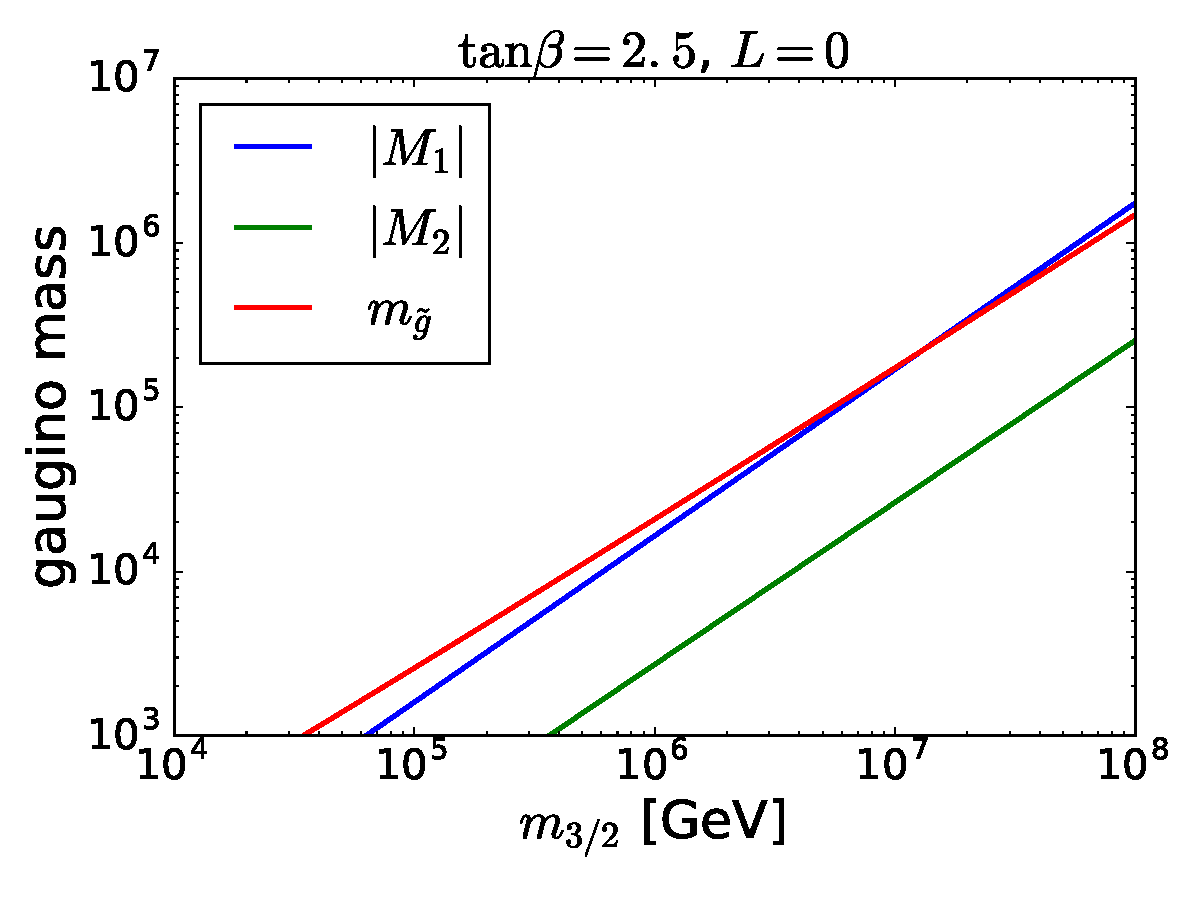
\includegraphics[width=0.48\hsize]{amsb_m32.pdf}
  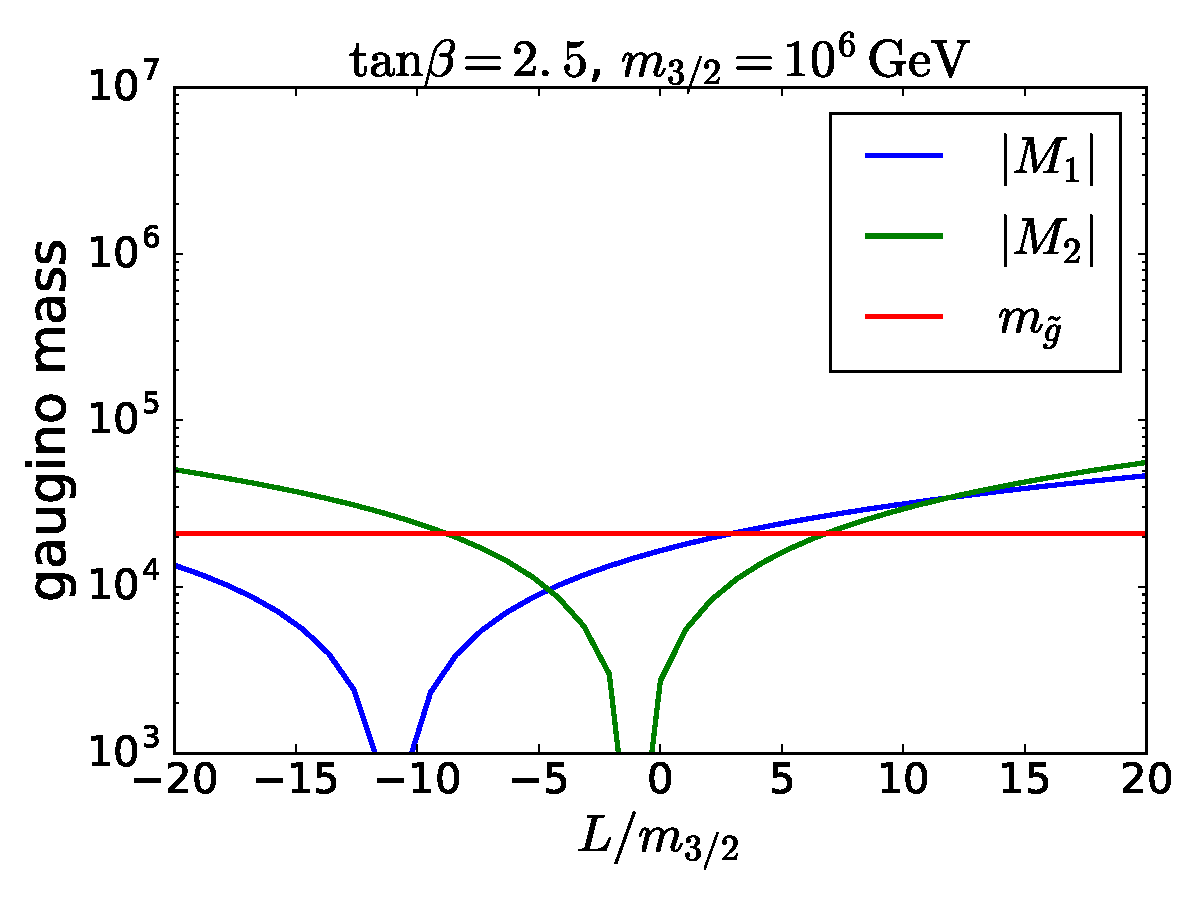
\includegraphics[width=0.48\hsize]{amsb_L.pdf}
  \caption{
    Gaugino masses as a function of $m_{3/2}$ with fixing $L = 0$ (left) and that of $L$ with fixing $m_{3/2} = 10^6\,\mathrm{GeV}$ (right).
    Blue, green, and red lines denote the masses of Bino, Wino, and gluino, respectively.
    $\tan\beta = 2.5$ is used in both figures.
  }
  \label{fig:amsb_spectrum}
\end{figure}

Below $M_S$, gaugino mass parameters further run towards the gaugino mass scale $M_{\tilde{G}}$, where the physical gaugino masses are determined.
Note that the bino and wino masses are roughly given by $|M_1 (M_{\tilde{G}})|$ and $M_2 (M_{\tilde{G}})$, while the gluino pole mass $m_{\tilde{g}}$ includes a sizable effect from the threshold correction as \cite{Giudice:2004tc}
\begin{align}
  m_{\tilde{g}} = |M_3 (M_{\tilde{G}})| \left[
  1 + \frac{g_3^2}{16\pi^2} \left( 12 + 9\ln \frac{M_{\tilde{G}}^2}{|M_3|^2} \right)
  \right].
\end{align}

In Fig.~\ref{fig:amsb_spectrum}, we show the dependence of gaugino masses on $m_{3/2}$ and $L$.
In the left panel, we take $\tan\beta = 2.5$ and $L=0$, and the $m_{3/2}$ dependence is shown.
Blue, green, and red lines denote the masses of Bino, Wino, and gluino, respectively.
We can see that, throughout the parameter region used here, Wino becomes the lighest gaugino, or the LSP that can be a dark matter candidate.
In this choice of parameters, $m_{3/2} = 10^6\,\mathrm{GeV}$ roughly corresponds to the observed value of the Higgs mass $m_h \sim 125\,\mathrm{GeV}$, which at the same time realizes the $\mathcal{O}(1)\,\mathrm{TeV}$ mass for Wino.
As we will see in Sec.~??, \rem{Caution!!} the Wino dark matter in this mass range is well-motivated since it gives us a collect relic abundance of the dark matter.

In the right panel of Fig.~\ref{fig:amsb_spectrum}, we also show the $L$ dependence of gaugino masses for $\tan\beta = 2.5$ and $m_{3/2} = 10^6\,\mathrm{GeV}$.
For simplicity, we neglect the relative phase of $m_{3/2}$ and $L$ and only consider the relative sign of them.
It can be seen that the hierarchy between gaugino masses is changed when a large value of $|L|$ is considered.
However, we can safely say that when the threshold correction is sufficiently small, $|L| \lsim \mathcal{O}(m_{3/2})$, Wino remains to be the LSP.
In addition, dependence of $m_h$ on $L$ is negligiblly small and $m_h$ changes only $\mathcal{O} (0.1)\,\mathrm{GeV}$ within the parameter choice of the right panel.


\subsubsection*{Dark matter and the R-parity}

\rem{Definition of LSP}


%%%%%%%%%%%%%%%%%%%%%%%%%%%%%%%%%%%%%%%%%%%%%%%%%%%%%%%%%%%%%%%%%%%%%%%%%%%%%%%
\subsection{Need review}
%%%%%%%%%%%%%%%%%%%%%%%%%%%%%%%%%%%%%%%%%%%%%%%%%%%%%%%%%%%%%%%%%%%%%%%%%%%%%%%

\begin{table}
 \centering
 \begin{tabular}{c|ccc|cc}
  & \multicolumn{3}{c|}{Quntum numbers} & \multicolumn{2}{c}{Masses}\\
  WIMP DM candidate & $SU(2)_L$ & $U(1)_Y$ & Spin & $m_\chi / \mathrm{TeV}$ &
  $\Delta m_\chi / \mathrm{MeV}$ \\
  \hline
  Higgsino & $2$ & $1/2$ & Dirac fermion & 1.1 & 341 \\
  Wino & $3$ & $0$ & Majorana fermion & 2.9 & 166 \\
  5-plet scalar & $5$ & $0$ & real scalar & 9.4 & 166 \\
  5-plet fermion & $5$ & $0$ & Majorana fermion & 10 & 166
 \end{tabular}
 \caption{Table of properties of popular WIMP DM
 candidates~\cite{Farina:2013mla, ArkaniHamed:2006mb, Hisano:2006nn,
 Cirelli:2007xd, Moroi:2013sla, Beneke:2016ync}.  The $SU(2)_L$
 electroweak charge, $U(1)_Y$ hypercharge, spin nature, mass, and mass
 difference compared with a charged component of the multiplet are
 shown.  See Sec.~\ref{???}  \rem{Caution!!} for the details of the last
 column.}  \label{tab_WIMP_property}
\end{table}

\rem{Relationship between $\lambda$ parameter above should be clearer}
WIMPs with mass around or just above the electroweak scale are
theoretically well-motivated in connection with problems of the SM such
as the naturalness problem.  For example, the minimal supersymmetric
extension of the SM (the so-called MSSM) contains several WIMP DM
candidate such as Higgsino and Wino.
Another example is the minimal dark matter (MDM)
model~\cite{Cirelli:2005uq, Cirelli:2007xd, Cirelli:2009uv}, which is a
simple extension of the SM with an $SU(2)_L$ electroweak multiplet such
as a $5$-plet scalar / fermion.  In these models, the stability of the
DM is ensured by the $R$-parity (for the MSSM case) and by high
dimensionality of the operator that describes the decay of the DM (for
the MDM case).  The properties of these WIMP DM candidates are
summarized in Table~\ref{tab_WIMP_property}.  The required masses to
explain the DM relic abundance through the freezeout mechanism are also
shown.  Since the non-relativistic annihilation cross section of
$\mathrm{TeV}$ mass particles is significantly enhanced by the
Sommerfeld enhancement effect~\cite{Hisano:2004ds, Hisano:2006nn}, there
are deviations from the rough estimation formula
Eq.~\eqref{eq_relic_abundance}.  We will return to this point later in
Sec.~\ref{???}.  \rem{Caution!!}  In addition, in the last column there
are mass differences $\Delta m_\chi$ between the DM and its charged
couterpart that will be explained in detail in Sec.~\ref{???}.
\rem{Caution!!}

%%%%%%%%%%%%%%%%%%%%%%%%%%%%%%%%%%%%%%%%%%%%%%%%%%%%%%%%%%%%%%%%%%%%%%%%%%%%%%%
\subsection{Minimal dark matter model}
%%%%%%%%%%%%%%%%%%%%%%%%%%%%%%%%%%%%%%%%%%%%%%%%%%%%%%%%%%%%%%%%%%%%%%%%%%%%%%%



\bibliographystyle{elsarticle-num}
\bibliography{../phd}

\end{document}
